\label{cha:requirements_analysis}

\section{Requirements Analysis}

\subsection{Derive Use Cases and Actors}
Goal of this task is to find four use cases and one actor according to the given story "Alice's Car Rental".

\begin{lstlisting}[
    caption={Use Case 1: "Rent a Car"},
    label={lst:car_rental_use_case_1},
    numbers=left,
    numberstyle=\tiny
]
    Title: Rent a Car
    Primary Actor: Customer
    Secondary Actor: None

    Preconditions:
        - Customer is registered and logged in
        - Customer has a valid drivers license and credit card

    Postconditions:
        - Customer has rented a car for the chosen time intervall

    Flow:
    1. The customer calls the application CarRental.
    2. The customer enters a start date and end date as the rental period
    3. The system shows a list with the cars which are available at the selected rental period
    4. The customer selects one of the listed cars
    5. The system shows a rental confirmation and stores the rental

    Alternative flows:
    3a. no cars are available at the selected time intervall
        3a1. The system shows a message that no cars are available at the selected time intervall and the flow continues from 2 or terminates
    4a. The customer does not want to rent any of the offered cars
        4a1. The flow terminates    
\end{lstlisting}



\begin{lstlisting}[
    caption={Use Case 2: "Registering Process"},
    label={lst:car_rental_use_case_2},
    numbers=left,
    numberstyle=\tiny
]
    Title: Registering Process
    Primary Actor: Customer
    Secondary Actor: None

    Preconditions:
        - Customer is not registered yet
        - Customer has a valid email address
        - Customer has a valid credit card and drivers license
        - Customer is at least 18 years old
        - Customer is not blacklisted by the car rental company or an insurance company

    Postconditions:
        - Customer is registered
        - Customer can rent a car
        - Customer can login to the car rental company's website

    Flow:
    1. Customer visits the car rental company's website or opens the app 
    2. Customer is asked to register or login
    3. Customer clicks on "Register"
    4. Customer is prompted for Email, name, drivers license, credit card number, date of birth
    5. A data validation is performed
    6. Customer needs to authenticate his email address
    7. Customer chooses a password and a username
    8. Customer shows a registration confirmation and the customer is registered successfully 

    Alternative flows:
    3a. Customer is already registered and clicks on "Login" instead of "Register"
    5a. Customer prompts false information or leaves non optional fields empty, so the data validation fails
        5a1. The customer is asked to fill out the form again
    6a. Customer does not authenticate his email address
        6a1. The customer will not be registered and the registration process is aborted
    7a. Customer chooses a username that is already taken
        7a1. The customer is asked to choose another username
    7b. The provided password does not fulfill the given criteria
        7b1. The customer is asked to choose a stronger password
\end{lstlisting}

\begin{lstlisting}[
    caption={Use Case 3: "Cancellation of a rental"},
    label={lst:car_rental_use_case_3},
    numbers=left,
    numberstyle=\tiny
]
    Title: Cancellation of a rental
    Primary Actor: Customer
    Secondary Actor: None

    Preconditions:
        - Customer has rented a car
        - Customer is logged in
        - Time interval of the rental has not started yet

    Postconditions:
        - Customer has cancelled the rental
        - Customer is prompted with a cancellation fee if neccessary

    Flow:
    1. Customer calls the application CarRental
    2. Customer clicks on "My Rentals"
    3. Customer selects the rental he wants to cancel
    4. Customer clicks on "Cancel Rental"
    5. Customer is prompted with a cancellation fee if neccessary
    6. Customer confirms the cancellation
    7. Customer is asked to confirm the cancellation again via email
    8. Customer confirms the cancellation via email
    9. Customer is prompted with a cancellation confirmation

    Alternative flows:
    3a. Customer has no rentals
        3a1. The system shows a message that the customer has no rentals and the flow terminates
    4a. Customer does not want to cancel the rental and the flow terminates
    5a. Customer does not want to pay the cancellation fee
        5a1. The flow terminates and the rental is not cancelled
    8a. Customer does not confirm the cancellation via email
        8a1. The flow terminates and the rental is not cancelled

\end{lstlisting}

\begin{lstlisting}[
    caption={Use Case 4: "Cancellation of the Registration"},
    label={lst:car_rental_use_case_4},
    numbers=left,
    numberstyle=\tiny
]
    Title: Cancellation of the Registration
    Primary Actor: Customer
    Secondary Actor: None

    Preconditions:
        - Customer is registered
        - Customer is logged in
        - Customer has no rentals or outstanding payments

    Postconditions:
        - Customer is not registered anymore

    Flow:
    1. Customer calls the application CarRental
    2. Customer clicks on "My Account"
    3. Customer clicks on "Cancel Registration"
    4. Customer confirmes the cancellation
    5. Customer is asked to confirm the cancellation again via email
    6. Customer confirms the cancellation via email
    7. Customer is prompted with a cancellation confirmation

    Alternative flows:
    3a. Customer has outstanding payments or rentals
        3a1. The system shows a message that the customer has outstanding payments or rentals and the flow terminates
    4a. Customer does not want to cancel the registration and the flow terminates
    6a. Customer does not confirm the cancellation via email
        6a1. The flow terminates and the registration is not cancelled
\end{lstlisting}

\subsection{Modelling the Use Case Diagram with UMLet}
The installation of the standalone version of UMLet is carried out as follows:
\begin{enumerate}
    \item Download the latest version of UMLet from \url{https://www.umlet.com/changes.htm}
    \item Extract the downloaded archive
    \item Run the executable file \texttt{umlet.sh} in the extracted folder
\end{enumerate}

A screendump of the folder structure of the extracted archive is shown in figure \ref{fig:umlet_folder_structure}.
\begin{figure}
    \centering
    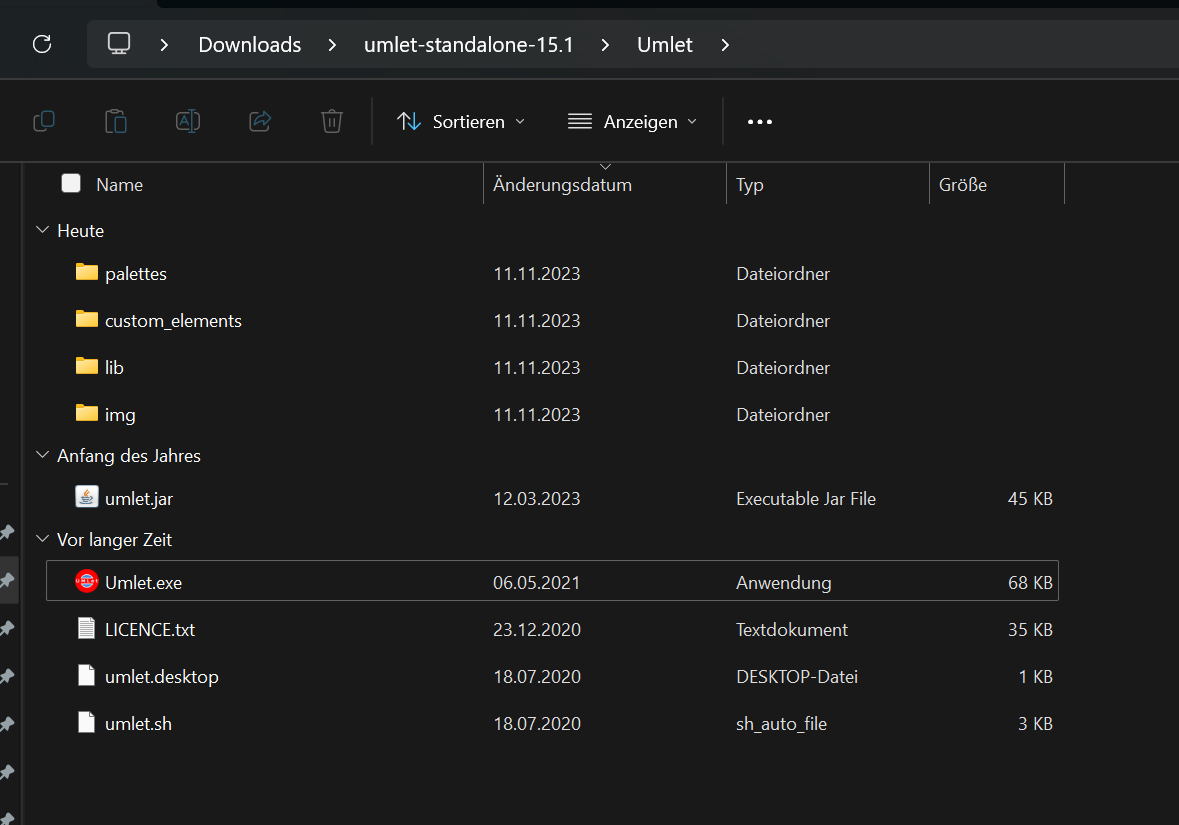
\includegraphics[width=0.8\textwidth]{figures/goLang/carRental/carRental_umletInstallation.png}
    \caption{Folder structure of the extracted UMLet archive}
    \label{fig:umlet_folder_structure}
\end{figure}

The use case diagram is shown in figure \ref{fig:car_rental_use_case_diagram}.

\begin{figure}
    \centering
    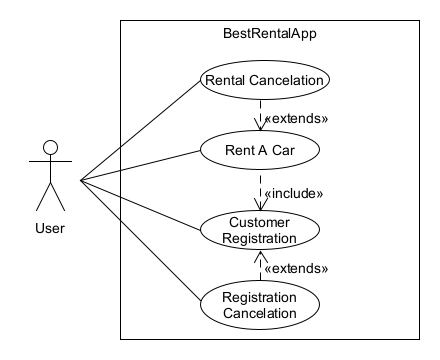
\includegraphics[width=0.8\textwidth]{figures/goLang/carRental/carRental_umlDiagram.png}
    \caption{Use case diagram of the car rental application}
    \label{fig:car_rental_use_case_diagram}
\end{figure}

\subsection{Alice's Car Rental}
\begin{lstlisting}[
    caption={Alice's version of Use Case 1},
    label={lst:alices_car_rental_use_case_1},
    numbers=left,
    numberstyle=\tiny
]
    1. Alice calls the application CarRental.
    2. Alice enters the 01.01.00 as a start date and 02.02.00 as the end date as the rental period
    3. The system shows a list with the cars which are available at the selected rental period
    4. Alice selects a VW ID.2
    5. The system shows a rental confirmation and stores the rental
\end{lstlisting}
